\documentclass{article}
\usepackage{graphicx} 
\usepackage{amsmath}
\usepackage{amssymb}
\usepackage[hidelinks]{hyperref}
\usepackage{subcaption}
\usepackage{tikz}
\usepackage{braket}
\usepackage{minted}
\usepackage{pseudo}
\usepackage{mathtools}
\usepackage{tabto}
\usepackage{float}
\usepackage{titlesec}
\usetikzlibrary{shapes.geometric}
\usepackage{lastpage}
\usepackage{tocloft}
\title{Peg Solitaire}
\author{
\centering
\begin{tabular}{c}
    Asmus Tørsleff\\
    qjv778@alumni.ku.dk (asmus.torsleff@gmail.com)\\
\end{tabular}}
\date{\today}
\begin{document}
\maketitle
\section{Introduction}
Peg solitaire is a game played on a board filled with holes. In these holes there can be a peg or no peg. If there is a peg with a neighbouring peg to one side and a hole to the opposite side, the neighbouring peg may jump over the middle peg and land in the hole on the other side. The middle peg is removed from the game after such a move. The objective of the game is to execute a series of moves such that you end up with as few pegs left on the board as possible. Wikipedia\footnote{\url{https://en.wikipedia.org/wiki/Peg_solitaire}} mentions previous attempts at solving the game, however I have not looked into these. I will be focusing on a variant of the game where the board is a line of $n$ holes. 
\section{Problem statement}
Given a board of length $n$ compute the amount of pegs in an optimal solution. 
We can use an $n$ bit binary number to represent the board, with ones where there are pegs. 


\textbf{Example:} The board 111 has available moves and so the amount of pegs in an optimal solution is 3.  The board 0111 has an available move and the amount of pegs in an optimal solution for this board is 2. 

\section{Solution approaches}

\subsection{Naive}
The first solution that comes to mind is to do a search though all possible sequences of moves, counting the number of pegs in each solution and returning the lowest one. 

\subsection{Dynamic programming}
After implementing the naive approach it is a small modification to add some kind of cashe to cut down on the branching in the search, this is sometimes refered to as memoization. 

\subsection{Domain knowledge}
For this board variant I have proven a few properties, see the pdf in the math part of the repository. One interesting property is that if there are 3 or more holes adjacent to each other we can handle the part of the board to each side of the holes as seperate and then just add the results together. Another is the fact that if there are $x$ pegs on the board and at least one hole, and all the pegs are adjacent then the optimal solution has $\lceil\frac{x}{2}\rceil$ pegs. Using the first fact we can devise an algorithm which uses a devide and concour strategy, and the second can spare us from exproing certain parts of the search tree. These are my contribution to this problem, granted someone might have come up with the same ideas. 

\section{Benchmarking}
I have implemented multiple solutions in C++ and run some benchmarks:
N implements the naive approach. 
M implements the dynamic programming approach. 
DN1+2 implements the naive approach, and takes advantage of both of the fracts from the domain knowledge section. 
DM1+2 implements the dynamic programming approach, and takes advantage of both of the fracts from the domain knowledge section. 
DM1 implements the dynamic programming approach, and takes advantage of only the devide strategy from the domain knowledge section. 

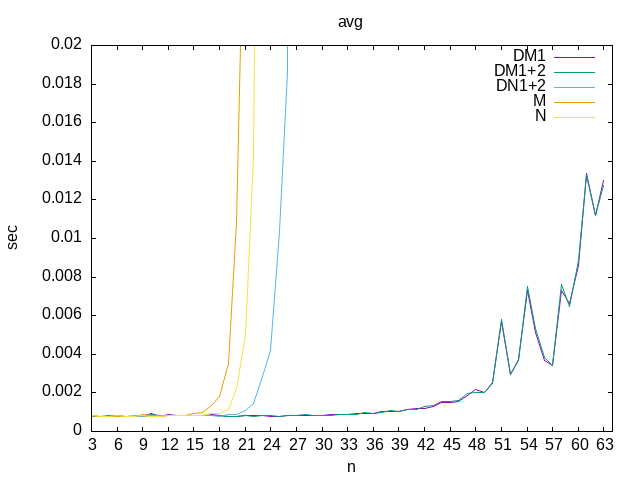
\includegraphics[width=\textwidth]{./cpp_comparison}
We can see here that DM1 and DM1+2 perform nearly identically, with DM1+2 being a bit slower on average, it seems the extra processing needed to check if the second fact can be applied is not worth it. We can also see that using the facts pressented makes it feasible to solve boards that are over twice as large. 
Curiously the dynamic programming approach does worse than the naive approach when running it in C++ with -O3 optimisation level. When implemented in Python it is better to use memoization. I suspect that if we were to reuse the cashe between runs the results would be better for this approach. 
The benchmark consists of generating 10.000 random boards for each board size, running all the programs on these boards and then taking the average time. 


\end{document}

